
\chapter{Introduction}
Traditionally health insurance in the US has been tied to employment through group plans. In 2013, only 17\% of Americans with private insurance\footnote{Non-private insurance is composed of Medicare, Medicaid and military health care} obtained it through the individual market \cite{census}. The differences between group and individual insurance are material for entrepreneurs leaving employment to start their own firms. Those that need coverage on the individual market face higher premiums or even the inability to purchase health insurance \cite{kaiser}. Uncertainty is also greater on the individual market; it is more likely for a person with an individual plan to lose insurance than someone under a group plan \cite{pauly}. 

Concerns over access to health care may be dissuading potential entrepreneurs from creating new firms. As one entrepreneur writes:
\begin{quote}
Obamacare affected me in another critical way as well. Its assurance of a stable insurance market that does not screen out someone with a preexisting condition made me far more comfortable starting my own business. It gave me a baseline of security that simply didn't exist before. It helped make entrepreneurialism possible. \cite{sullivan}
\end{quote}

The literature on this topic focuses on answering how potential entrepreneurs are affected by access to health insurance. Early work by Holtz-Eakin, Penrod and Rosen \cite{holtz_health}  estimated the propensity to become self-employed as a function of access to health insurance. More recent work refined these types of estimates for specific sub-populations; Fairlie, Kapur and Gates \cite{fairlie_health} is an example that uses different datasets to generate estimates by sex and for workers nearing retirement. We are deepening our understanding of how access health insurance impacts various types of entrepreneurs. 

We are not aware of research asking the complementary question of what potential \emph{enterprises} are affected by access to health insurance. To illustrate, consider the response of one high-tech entrepreneur in Cambridge, MA when probed about the entrepreneurial impact of the 2006 health insurance reform in Massachusetts:
\begin{quote}
[The] top barrier[s] to people starting companies are [a] lack of drive and lack of capital ... it takes a lot of drive to start companies, and lack of health care is too small a barrier compared to others. For some freelancer[s] I think health care does help.
\end{quote}
The above quote suggests we will see an effect in single person consulting companies but not in high growth startups. More generally, the impact of health care reform may vary by type of firm and not just by type of entrepreneur. 

In this paper we contribute to the literature in two ways. First, we show by example that using heterogeneity in firm characteristics can increase our ability to produce significant results in otherwise challenging quasi-experimental settings. Second, our example results are interesting in their own right; they broaden our understanding of what influences the rate of entrepreneurship. 

Specifically, we take advantage of variation in the two requirements for entrepreneurship called out in the above quote: drive and capital. We use a firm's tax status to generate insights about drive; higher tax rates should reduce overall incentives to start firms and therefore mitigate entrepreneurial drive. We also develop a theoretical model that shows how start-up capital requirements can inform us about whether entrepreneurs are in fact constrained by access to health care. Our results suggest that while health care reform may provide marginal benefits to general entrepreneurship and stronger benefits to non-profit entrepreneurship, in general health care is not a effective policy lever to influence the level of entrepreneurship in an economy.

The rest of the article proceeds as follows. Section \ref{sec:review} reviews our current knowledge on the importance of both access to health care and entrepreneurship. Section \ref{sec:reform} describes the Massachusetts health reform we use as a policy shock. Section \ref{sec:model} outlines a model that considers how the reform should heterogeneously affect entrepreneurship by industry. Section \ref{sec:data} describes the data sources we use in our analysis. Section \ref{sec:regression} explains our empirical approach. Section \ref{sec:results} presents the effects of the reform on entrepreneurship and Section \ref{sec:conclude} concludes. 

\chapter{Literature Review}
\label{sec:review}

The importance of health insurance to economic rather than pure health outcomes was first explored by labor market researchers. Their motivation was to understand what is commonly referred to as ``job lock'': inefficiencies in matching workers to jobs due to non-portable benefits. Early findings suggested job lock due to health insurance was significant. Madrian \cite{madrian} for example estimated that health insurance job lock reduced voluntary turnover by 25\%. More recent work has continued to find significant results with real implications for policy makers. Garthwaite et al. \cite{garthwaite} argue that providing free health insurance to poor, childless Americans is a bad idea; they estimate it would reduce the US labor force by over half a million workers. 

Entrepreneurship researchers shifted the scope of this investigation by in effect asking: we know health care matters for labor markets, but what about new firm creation? This is arguably an equally important economic outcome to consider, for example Haltiwanger et al. \cite{haltiwanger} has recently pointed out that startups account for a disproportionate amount of new job creation in the US. However in contrast to the job lock literature, the study of entrepreneur lock has produced less consistent results. 

Holtz-Eakin et al. \cite{holtz_health} were the first to ask this question and found no strong relationship using both variance in spousal insurance coverage and the COBRA regulation\footnote{Consolidated Omnibus Budget Reconciliation Act (COBRA) of 1985} requiring the ability to continue coverage after employment ends. More recent work by Bailey \cite{bailey} also finds no result using the 2010 Affordable Care Act as a shock which exogenously provided health insurance to dependents under 26 years old. 

In contrast, both Wellington \cite{wellington} and Fairlie et al. \cite{fairlie_health} provide evidence that having a spouse with insurance increases the propensity to become an entrepreneur. Fairie et al. \cite{fairlie_health} also exploit the Medicare cutoff at age 65 to suggest entrepreneurship increases at the discontinuity. Olds \cite{olds} targets entrepreneurs with children and finds providing health insurance to previously uninsured children increases self-employment rates in the household by 23\%.  Becker and Tuzemen \cite{tuzemen} apply census data to the 2006 health care reform in Massachusetts and estimate that a 1\% increase in health insurance rates generates a 0.06\% increase in the self-employment rate. 

There has also be cases where the results have been negative. Heim and Lurie \cite{heimLurie} analyze tax filing data using the same 2006 health care reform in Massachusetts. They find a small decrease in the overall probability a taxpayer earns the majority of their income from self-employment.

These results tell us that entrepreneurship lock may be a more subtle phenomenon than job lock and manifest differently across sub-populations given the policy environment. We think more progress could be made in this area if researchers augmented their approaches with information about the characteristics of firms created by their chosen policy shock or matching method. 

Our first example of using firm characteristics relies on the contrast in tax treatment between non-profit and for-profit firms. A number of studies have found a strong, negative relationship between between tax rates and the decision to become an entrepreneur. Gentry and Hubbard \cite{gentry} use US Census panel data to estimate how changes in effective marginal tax rates impact the propensity for an individual to become self-employed and find a significant effect. Overall their dataset has about 3\% of individuals entering self-employment over the panel time period; they estimate a 5\% increase in tax rates lowers the probably of self-employment to around 2.75\%. Cullen and Gordon \cite{cullen} build a theoretical model that enables them to identify various channels linking tax rates to entrepreneurship and use income tax data to find a large effect on risky businesses that incur losses early on. Da Rin \cite{darin} uses firm level panel data for Western Europe and finds drops in corporate tax rates increases firm entry. Djankov et al. \cite{djankov} finds similar results with a global set of countries. 

Our second example of firm characteristics relies on the consensus that many entrepreneurs are in fact constrained by the lack of access to capital. Evans and Jovanovic \cite{evans} is one of the early works that tied wealth to higher entrepreneurial rates. Holtz-Eakin et al. \cite{holtz_capital} use inheritance size as way to further explore capital constraints on entrepreneurship; they find the probability of entrepreneurship and amount of capital used in the firm to increase with inheritance size. More recent work also using inheritances by Hurst and Lusardi \cite{hurst} confirms the positive relationship between wealth and entry. 

We apply this approach of using firm characteristics to the Massachusetts reform of 2006. We believe the setting is appropriate because prior work on health outcomes have provided evidence that the policy change has made a real impact on the health insurance market in Massachusetts. Toussaint et al. \cite{toussaint} find uninsurance rates dropped in trauma centers. Miller \cite{miller_er} shows non-urgent ER visits dropped after the reform. As mentioned above, our setting has also led to conflicting estimates on entrepreneurial impact by different authors. We believe our approach is especially helpful in these kinds of settings with ambiguous results. 

\chapter{Reform in Massachusetts}
\label{sec:reform}


In late 2006, the state of Massachusetts passed a law entitled ``An Act Providing Access to Affordable, Quality, Accountable Health Care''. The act was motivated by a number of concerns, including:

\begin{enumerate}
\item Reducing the number of uninsured residents, which had been steadily increasing in the period from 2000 to 2004 \cite{bisweek}
\item Addressing the public cost of providing health care to uninsured residents \cite{npr}
\item Restructuring a federal waiver that allocated funds to Massachusetts for uncompensated care \cite{heritage}
\item The highest individual (non-group) health insurance costs in the nation \cite{gruber_mass}
\end{enumerate}

The act resulted in a number of changes to the health care industry between 2006 and 2007. Provisions included a mandate that required all adult residents to purchase health insurance conditional on affordability guidelines, health insurance subsidies to lower income families, a state run marketplace for individual insurance, a tax on larger employers that declined to provide health insurance to employees and the expansion of the state's Medicaid program for children. Much of the act was phased in over time as seen in Figure \ref{fig:reformTimeline}.

\begin{figure}[h]
	\centering
	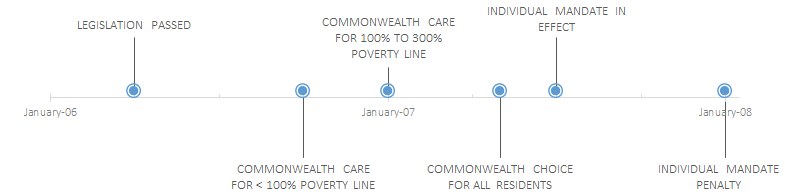
\includegraphics[width=\textwidth]{resources/timeline}
	\caption{Timeline of plans available for individual purchase and mandate requirements}
	\label{fig:reformTimeline}
\end{figure}

A net effect of the act was a drop in uninsured Massachusetts residents. The Massachusetts Health Insurance Survey is conducted in the first half of each year and asks about the current insurance status of Massachusetts residents. It suggests that the act resulted in an approximate 60\% reduction in uninsured adult residents. Figure \ref{fig:uninsuredRate} illustrates the effect by contrasting the periods before and after the law was fully implemented. 

\begin{figure}[h]
	\centering
	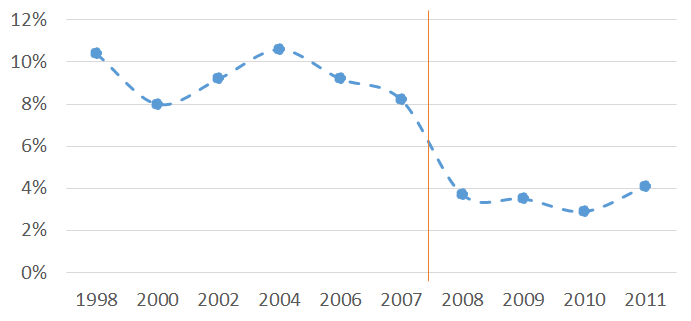
\includegraphics[scale=0.6]{resources/uninsured}
	\caption{Percent of Massachusetts residents uninsured between the ages of 19 to 64}
	\label{fig:uninsuredRate}
\end{figure}

From an entrepreneurial standpoint, we view the act as having improved the health insurance marketplace for self-employed residents. We are agnostic to the mechanism. One possibility is the lower cost of insurance; Gruber \cite{gruber_mass} suggests that controlling for plans with lower benefits, the cost of individual insurance plans dropped by 20\% as a results of the reforms. Other potential mechanisms include the ability to sign up for plans with preexisting conditions and greater confidence in keeping insurance conditional on becoming sick. We use the period starting in 2008 as the treatment period for the shock since the law's main effect of lowering the uninsured rate was observed in 2008. 

Massachusetts historically had a low rate of uninsured residents relative to the rest of the United States. Between 1999 and 2006, Census CPS estimates the Massachusetts had on average a 9.4\% uninsured rate. The US as a whole had an average 14.7\% rate over the same time period. As a result, we think the state of Massachusetts is a relatively strong setting to test our hypotheses; potential entrepreneurs were more likely to face a real choice to give up their current health insurance coverage in order to start firms. In a state like Texas with a 23.6\% uninsured rate, there are likely to be more potential entrepreneurs that lack insurance prior to starting their firms so we would have a weaker instrument to measure our desired effect. 

Simultaneity is a concern in our setting. We can imagine there exists both a supply of individuals willing to become an entrepreneur as well as a demand for entrepreneurs in the form of opportunities for entrepreneurship. We assume the health care reforms have a minor impact on opportunities for entrepreneurship outside of the health care industry in our analysis. The assumption would be false if for example the health reform freed up enough disposable income to significantly increase spending on restaurants. Holding our assumption enables us to identify how the health care law changes the supply of entrepreneurship. 

\chapter{Theoretical Motivation}
\label{sec:model}

\section{Aggregate Effect}

We will use this empirical context to test four propositions. First, building on Gruber and Madrain \cite{gm2002}, consider a compensating differential model of a worker that currently has health care through their job but expects to be unable to attain health care as an entrepreneur. Utility is a function of both returns to an activity and a binary indicator of health insurance coverage. We can imagine the returns to an activity being dependent on tangible characteristics such as wages as well as less tangible ones such as job satisfaction. Workers stay at the firm as long as the return to employment $w$ and the return to entrepreneurship $r$ as such that
$$U(w,1) \ge U(r,0)$$

If there is a shock that creates a market for non-group health insurance at utility cost $c$, the worker will stay are long as
$$U(w,1) \ge \max\{U(r,0),U(r-c,1)\}$$

This should shift some mass of workers to become entrepreneurs as long as some workers value health insurance more than the cost on the non-group health market and for those workers
$$U(w,1) < U(r-c,1)$$

So this model would predict that the health-care shock increases entrepreneurship. 

\textbf{Proposition 1:} 
Improving access to health-care should increase entrepreneurship. 

\section{Tax Heterogeneity}

However, the reform in Massachusetts also involved changes to government expenditure. In 2013, 30\% of the Massachusetts budget was spent on the Mass Health \cite{masshealth} subsidy program. This may have affected the expected return $r$ to self-employment conditional on creating a successful firm if for example entrepreneurs believed the subsidies would eventually be paid for by a higher progressive tax on earnings.

This could be viewed as a mitigating the effect of the shock on self-employment. Now workers will leave if the utility change in taxes $t$ is such that

$$U(w,1) < U(r-t-c,1)$$

These expectations should affect incentives to create non-profit firms differently than for-profit firms. In the above model utility is decreasing in taxes so non-profit firms should gain more from the reform so we should see a heterogeneous effect of the shock across these two types of firms.  

\textbf{Proposition 2:} 
The health care reform package should cause a relatively larger increase in non-profit firms than for-profit firms. 

Note we are assuming that the utility cost of health insurance, $c$, is the same for non-profit and for-profit entrepreneurs.  

\section{Capital Heterogeneity}

Our next proposition considers another form of industry based heterogeneity. Suppose a potential entrepreneur is considering to start a new venture. Conditional on having an opportunity, factors such as ability to attract complementary talent \cite{stuartSorensen} can impact the decision to execute the venture. We can model the probability of starting a firm as the probability of getting an opportunity that fits the constraints binding the entrepreneur. 

Suppose two such constraints are the capital required to start the firm and access to health care  outside of current employment. An opportunity can vary on both dimensions. Some ideas can of course require more capital to execute than others. Additionally, some ideas could be worked on without leaving existing employment. For example, survey data suggests half of all software developers create applications outside of their formal employment \cite{evans}. Also, the constraints are likely to vary by individual. Individuals vary in their social networks which can influence access to capital \cite{uzzi}. A potential entrepreneur may be relatively less constrained by health care if her spouse's employer provided health insurance for their family. 

\textbf{Proposition 3:} 
Suppose opportunities to start low capital firms are at least as common as high capital firms. Then improving access to health care should increase the probability of starting a low capital firm relative to a high capital firm. Equality or a negative difference between the low and high capital groups suggests low capital opportunities are strongly constrained outside of access to health care. 

\textbf{Proof:}
See Appendix A for a formal statement of the proposition, its required assumptions and its proof. 

The intuition behind Proposition 3 can be conveyed in the single entrepreneur case using a visualization of the space of potential opportunities. Suppose an entrepreneur has a level $\alpha_i$ of health care and level $\beta_i$ of capital to start with. The entrepreneur can then execute opportunities that require at most those levels of resources. The shaded region in Figure \ref{fig:ideaSpace} represents the space of opportunities executable by the entrepreneur. If we think of the health care reform as shifting level $\alpha_i$ to $\alpha_i'$, the striped region's set of opportunities also become feasible. Note that only opportunities with resource requirements lower than $\beta_i$ are affected by the shift in resource $\alpha$. As long as there is not a larger mass of potential opportunities that require high capital than low capital, when we sum across all individual entrepreneurs we should see more executed opportunities with low capital than high capital. 

\begin{figure}[h]
	\centering
	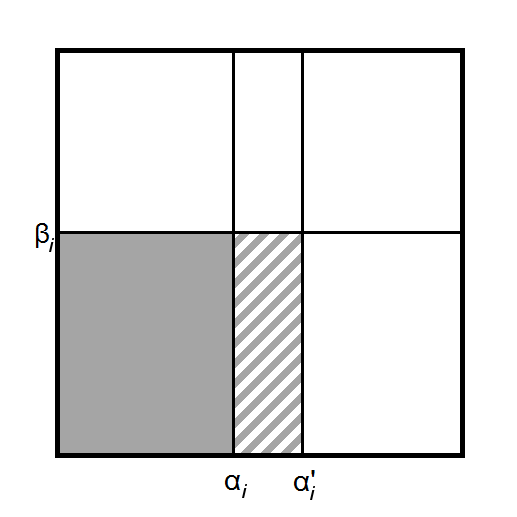
\includegraphics[scale=0.5]{resources/Prop1}
	\caption{Subset of opportunity space executable by agent $i$ with resources $(\alpha_i,\beta_i)$ versus$(\alpha_i', \beta_i)$.}
	\label{fig:ideaSpace}
\end{figure}

\chapter{Data Sources}
\label{sec:data}


We measure our outcome variable of entrepreneurship with two different US Census data sets. First we focus on self-employment as measured in the American Community Survey (ACS). The ACS surveys households for employment status and provides information on self-employment rates on a county basis. Although this self-employment data lacks the industry classification necessary for main findings, it connects well with previous research that estimated the impact of health reform on self-employment rates. 

To test our hypothesis related to industry characteristics, we use the Nonemployer Statistics (NS) series also from the US Census. The NS is based on tax filings and includes self-employed individuals as well incorporated businesses and partnerships that lack employees. 

Both of our data sources suffer from being measurements of net rather than gross values. For example, if  we do not obverse a change in number self-employed individuals over a period of time, this does not necessarily mean no new enterprises were created. No change happens when the rate of establishment entrance equals the rate of firm establishment. Exit and entrance are also definitional; a previously existent firm that hired its first worker would be listed as a exit in the NS data one year but an entrant in a following year if that worker was later laid off. Unfortunately we were not able to find a satisfactory public data set with gross establishment or firm numbers. However we think any change in the rate of entrepreneurship will still manifest in our dataset. To illustrate, figure \ref{fig:construct} shows how the number of nonemployers changes in construction, a traditionally cyclical industry. We see a rise during the boom period of mid-2000 followed by a fall after the 2008 recession. 

\begin{figure}[h]
	\centering
	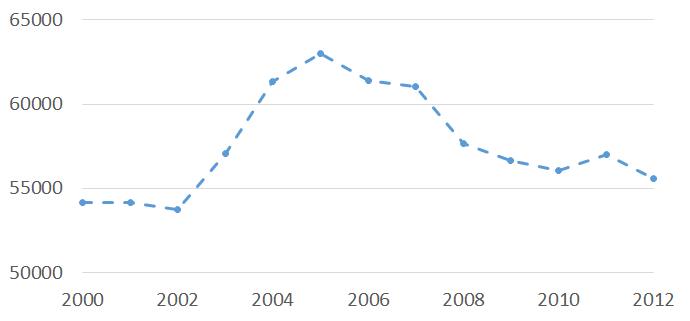
\includegraphics[scale=0.6]{resources/construction.png}
	\caption{Number of nonemploying construction firms in Massachusetts}
	\label{fig:construct}
\end{figure}

Table \ref{tab:basic} provides summary statistics for our variables of interest in Massachusetts and other New England states from 2000 to 2012. To reduce potential endogeneity we remove firms in the health care industry from our dataset. The rest of New England is approximately similar to Massachusetts in size and establishment characteristics although Massachusetts is more urban than the rest of New England. 

\begin{table}[h]
	\centering
	\caption{Summary statistics for Massachusetts and other New England states}
	\begin{tabular}{lrr} \hline \hline
& Massachusetts  & Other New England  \\  \hline
Population &   6,431,559 &    7,847,646 \\
Percent Urban &        91.09\% &        60.91\% \\
Percent Uninsured &        13.50\% &        13.74\% \\
Percent Aged 20 to 24 &         6.40\% &         5.94\% \\
Percent of Households with Children &        30.60\% &        31.68\% \\
\hline \textbf{Self-Employment} & & \\
Number &      210,684 &      311,317\\
Percent of Population &       3.28\% &       4.01\% \\
Yearly Change in Percent of Population &         -0.01\% &         -0.02\% \\
\hline \textbf{Non-employers} & & \\
Number &      423,846 &      572,954\\
Percent of Population &       6.39 \% &       7.15 \% \\
Yearly Change in Percent of Population &          0.06 \% &          0.07 \% \\
 \hline \hline \end{tabular}

	\label{tab:basic}
\end{table}

In order to measure the effect of the health care reform on entrepreneurship, ideally we would want to measure change in probability that an individual becomes an entrepreneur. Given that our dataset that lacks observations of individuals, we focus on the changes in our variables of interest. For our first proposition, we measure this as the change in percentage of self-employed people per county ($Change_{ct}$). For our other propositions, we measure the change in non-employed establishments per million people in each county ($Change_{cit}$) by industry. The large number of 4 digit NAICS classifications causes us to use the million people denominator; simple percentages would lead to coefficients that become cumbersome to read. 

\chapter{Empirical Approach}
\label{sec:regression}

\section{Overall Impact}

Proposition 1 suggests we should see an increase in entrepreneurial activity after the health care reform. To test this prediction, we first apply a difference in differences approach with counties in Massachusetts as the treatment group and various controls. If the reform improved the return to entrepreneurship for some workers, our treatment indicator should be positive. 
\begin{align}
Change_{cst} = \alpha_c + \zeta_s + \delta_t + \beta \, \mathbf{1}\{\text{county in MA}\} \cdot \mathbf{1}\{\text{year > 2007}\} + \epsilon_{cst}
\end{align}

Here $Change_{cst}$ represents the change in our variable of interest per million residents in year $t$ and county $c$ of state $s$. The model includes fixed effects for year ($\delta$), county ($\alpha$) and state ($\zeta$).

Our first control consists of counties in New England outside of Massachusetts. We define New England as Connecticut, Maine, New Hampshire, Rhode Island, Vermont and Massachusetts. This helps account for broad regional shocks such as recessions that affect all of New England. 

For a more targeted approach, we use border matching as our second control. Here our treatment group consists of Massachusetts counties that share a border with another state. This pulls out the cities of Boston and Cambridge. Our control group consists of counties in Connecticut, New Hampshire, Rhode Island, Vermont and New York that border Massachusetts. We would expect this method to help ensure our control and treatment groups are similar if geographically close counties  have for example more similar economic activity than distant counties. 

Finally we employ a synthetic control method drawing on counties across all US states other than Massachusetts. Our approach mirrors the procedure used in Abadie et al. \cite{abadie} although we slightly modify their source code to better account for rounding errors in our specific use case. For each county in Massachusetts we generate a synthetic pair as a control. We first prune the matching pool by removing counties that strongly differ from the Massachusetts county in either level of urbanization, uninsured rate, population age, or the frequency of children in a household. We then assign weights to the pruned set of counties in order to minimize the difference in our outcome variable between control and treatment before our shock. This has the benefit of removing any pre-trend from our natural experiment as seen in Figure \ref{fig:state_contrast}. The downside is that the matching is done algorithmically and may produce counterintuitive controls. In our case the procedure yielded arguably valid results; self-employment rates in Boston (Suffolk County, MA) before 2008 most closely matched a combination the counties for Ann Arbor, MI (57\% weight), Lexington, KY (25\% weight) and other various counties across the US. 

\begin{figure}[h]
	\centering
	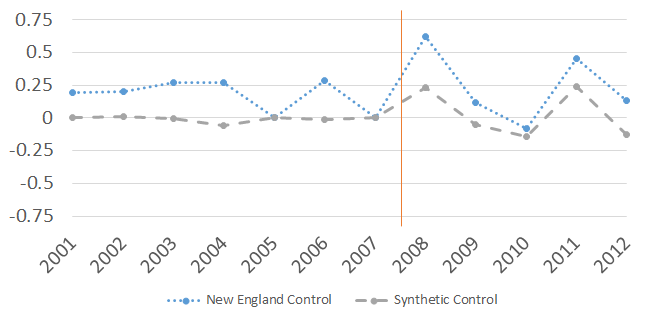
\includegraphics[scale=0.6]{resources/ne_synth.png}
	\caption{Yearly Treatment Effect Point Estimates for Self-Employed Individuals}
	\label{fig:state_contrast}
\end{figure}

\section{Non-profit Heterogeneity}

Proposition 2 predicts that non-profits were more strongly impacted by the health care reform since there is no long term cost of increased taxes that balances the short term benefit of health care access. To test this prediction, we use Economic Census data that provides information about the number of tax paying and tax-exempt establishments at the 4 digit NAICS code industry level for a subset of industries.  

Our first specification restricts our observations to counties in Massachusetts. For each of our industries we use the percentage of the industry's firms that were excluded from federal taxes as a measure of treatment intensity. 

\begin{align}
Change_{cit} = \alpha_c + \gamma_i + \delta_t + \beta \times \{\text{\% of industry non-profit}\} \cdot \mathbf{1}\{\text{year > 2007}\} + \epsilon_{ct}
\end{align}

Here $Change_{cit}$ represents the number of net new establishments created per million residents in year $t$, county $c$ and industry $i$. The model includes fixed effects for year ($\delta$), county ($\alpha$) and industry ($\gamma$). Although our observations are based on NAICS codes at the 4 digit level, we apply fixed effect $\gamma$ at the 2 digit NAICS code level in order to have a manageable number of coefficients to estimate given the constraints of our data set. Since our self-employment data set lacks industry information we only apply model (2) to our non-employer data set. 

Model (2) leaves open the possibility of another shock happening at the same time that also differentially affected non-profit industries. The results would be invalid if for example the 2008 recession was relatively milder for non-profit firms than for for-profit firms. To control for this, we extend our approach to a triple difference model which should account for shocks that both affected Massachusetts and our synthetic control. 
\begin{align}
Change_{cit} = & \; \gamma_i \cdot \alpha_c + \gamma_i \cdot \delta_t +  \alpha_c \cdot \delta_t \nonumber   \\
& + \beta  \times \{\text{\% of industry non-profit}\} \cdot \mathbf{1}\{\text{year > 2007}\}  \cdot \mathbf{1}\{\text{county in  MA}\} \nonumber  \\
& + \epsilon_{ict}
\end{align}



\section{Capital Requirement Heterogeneity}

Proposition 3 states that as long as opportunities for low capital entrepreneurship are at least as prevalent as opportunities for high capital entrepreneurship, we should see that the health insurance shock increased low capital entrepreneurship relative to high capital entrepreneurship. We first test this proposition using model (4) within Massachusetts. 
\begin{align}
Change_{cit} =  \alpha_c + \gamma_i+ \delta_t + \beta \, \mathbf{1}\{\text{low capital industry}\} \cdot \mathbf{1}\{\text{year >= 2008}\} + \epsilon_{ict}
\end{align}
Our observation count of industries across counties is large enough for us to deploy industry fixed effects $\gamma$ at the 4 digit NAICS code level. 

We use the Survey of Business Owners (SBO) Public Use Microdata Sample (PUMS) from 2007 to determine which industries have low capital requirements. Since the SBO PUMS data only reports on 2 digit NAICS codes, we calculate the percentage of businesses that required less than \$1000 of startup capital for each 2 digit NAICS code and match the 2 digit NAICS codes with our 4 digit industry codes. Because we lack resolution of our treatment at the 4 digit industry code level, we avoid treatment intensity here in contrast to our non-profit approach. We consider industries above the middle of the range of percentages as low capital industries. The PUMS data provides the capital requirements by employment size so we customize our calculation of low capital industries for firms with no employees. 

Model (4) leaves open the possibility of another shock happening at the same time that also differentially affected low capital industries. We therefore include the triple difference model (5). 
\begin{align}
Change_{cit} = & \; \gamma_i \cdot \alpha_c + \gamma_i \cdot \delta_t +  \alpha_c \cdot \delta_t \nonumber   \\
& + \beta \, \mathbf{1}\{\text{low capital industry}\} \cdot \mathbf{1}\{\text{year >= 2008}\}  \cdot \mathbf{1}\{\text{county in MA}\} \nonumber  \\
& + \epsilon_{cit}
\end{align}

\section{Inference}

Fixed effects with errors clustered by state is the usual approach to inference when dealing with state wide shocks. However as pointed out by Donald and Lang \cite{donald}, inference with a small number of cluster groups can suffer from large bias. In our New England control specification we only have 5 groups. We also have limited observations per group; each New England state just has 11 counties on average so the two-step approach suggested by Donald and Lang does not apply. In addition, our shock only applies to a single state cluster leading to a singular covariance matrix under our modeling specification; see Appendix B for an illustration with a simple linear model. 

To address these concerns, we use a Monte-Carlo simulation described in Appendix C to test various inference approaches conditional on the properties of our dataset. As a result, we report confidence intervals based on Huber-White errors. 

\chapter{Findings}
\label{sec:results}

\section{Importance of Control Group}

Table \ref{tab:control} summarizes our first finding as a test of Proposition 1. We run the difference in difference model (1) against the yearly percentage change in self employed population. Over our period of interest, about 3.29\% of Massachusetts' population was unincorporated, self employed individuals. Our column 1 result suggests the percentage of self-employed residents increased by 0.08 per year as a result of health care reform, for an overall increase of 0.4\% by the end of our period of interest. This result compares well to the Becker and Tuzemen \cite{tuzemen} result of 0.6\% which measured the impact of the same shock on self employment using an IV approach on aggregate state data. 

However we find the magnitude of our results to be sensitive to the control group in use. Column 2 uses the border county procedure to attempt a closer match between our treatment and control groups. Column 3 uses the synthetic control group process. Both results in similar standard errors but magnitudes that are not distinguishable from zero. 
\begin{center}
	\begin{table}[h]
		\centering
			\caption{Diff-in-diff estimator of yearly percentage change in self-employment} 
		{
\def\sym#1{\ifmmode^{#1}\else\(^{#1}\)\fi}
\begin{tabular}{l*{3}{c}}
\hline\hline
          &\multicolumn{1}{c}{(1)}&\multicolumn{1}{c}{(2)}&\multicolumn{1}{c}{(3)}\\
\hline
Massachusetts $\times$ Post 2007&    0.075** &    0.063   &    0.040   \\
          &  (0.030)   &  (0.037)   &  (0.031)   \\
[1em]
Year FE   &      Yes   &      Yes   &      Yes   \\
[1em]
State FE  &      Yes   &      Yes   &      Yes   \\
[1em]
County FE &      Yes   &      Yes   &      Yes   \\
\hline
\(N\)     &      804   &      264   &      336   \\
\(R^{2}\) &    0.050   &    0.136   &    0.109   \\
Control   &New England   &Border Counties   &Synthetic   \\
Weight    &Population   &Population   &Population   \\
\hline\hline
\multicolumn{4}{l}{\footnotesize Standard errors in parentheses}\\
\multicolumn{4}{l}{\footnotesize * p<0.10, ** p<0.05, *** p<0.01}\\
\multicolumn{4}{l}{\footnotesize Diff-in-diff model of health care reform from 2000 to 2012 with Massachusetts treated after 2007. }\\
\multicolumn{4}{l}{\footnotesize Maine, Connecticut, Vermont, Rhode Island and New Hampshire used as controls in column (1). }\\
\multicolumn{4}{l}{\footnotesize Column (3) uses a synthetic control model that matches each Massachuetts county pre-trend against}\\
\multicolumn{4}{l}{\footnotesize \space US counties with similar income, age, urban and insurance rate characteristics. }\\
\end{tabular}
}
	
		\label{tab:control}
	\end{table}		
\end{center}

We interpret these findings to mean any possible effect our shock had on self-employment is likely to be too small to detect using the publicly available census data on individuals. We believe the sensitivity to control explains why the Becker and Tuzemen \cite{tuzemen} results differ from the Heim and Lurie results \cite{heimLurie}. 

\section{Long Run Tax Impact}

Table \ref{tab:nonprofit} shows our results testing Proposition 2 claim that non-profit firm creation should increase faster than for-profit firm creation. Column 1's results from running model (2) suggests a noticeable effect, which remains once we apply the triple difference specified in model (3) with the New England and synthetic controls. Although our estimate under border control loses its significance, we believe the is an artifact of poor matching; services such as homeless shelters appear in our dataset for Massachusetts border counties but not in the border control group. 

The magnitude of our observed effect is large. Our estimate suggests that an industry composed only of non-profits would gain about 52 new firms per million people each year relative to an industry composed only of for-profit firms. To contrast, our dataset shows on average 13 new firms were created per million people each year for a typical industry. 

\begin{table}[h]
	\footnotesize
	\centering
	\caption{Impact of health reform on non-profit non-employers}
	{
\def\sym#1{\ifmmode^{#1}\else\(^{#1}\)\fi}
\begin{tabular}{l*{4}{c}}
\hline\hline
          &\multicolumn{1}{c}{(1)}&\multicolumn{1}{c}{(2)}&\multicolumn{1}{c}{(3)}&\multicolumn{1}{c}{(4)}\\
\hline
\% Non-profit $\times$ Post 2007&   42.565***&            &            &            \\
          &  (9.203)   &            &            &            \\
MA $\times$ \% Non-profit $\times$ Post 2007&            &   52.015***&   20.728   &   52.550***\\
          &            & (14.387)   & (18.712)   & (12.941)   \\
County $\times$ Year FE &       No   &      Yes   &      Yes   &      Yes   \\
Industry $\times$ Year FE &       No   &      Yes   &      Yes   &      Yes   \\
County $\times$ Industry FE &       No   &      Yes   &      Yes   &      Yes   \\
Year FE   &      Yes   &       No   &       No   &       No   \\
County FE &      Yes   &       No   &       No   &       No   \\
State FE  &      Yes   &       No   &       No   &       No   \\
Industry FE &      Yes   &       No   &       No   &       No   \\
\hline
\(N\)     &     3288   &    10560   &     4236   &     6384   \\
\(R^{2}\) &    0.019   &    0.143   &    0.121   &    0.131   \\
Control   &Within MA   &New England   &Border Counties   &    Synth   \\
\hline\hline
\multicolumn{5}{l}{\footnotesize Standard errors in parentheses}\\
\multicolumn{5}{l}{\footnotesize * p<0.10, ** p<0.05, *** p<0.01}\\
\multicolumn{5}{l}{\footnotesize Column (1) is a diff-in-diff model of non-employers per million people in Massachusetts from  }\\ 
\multicolumn{5}{l}{\footnotesize \space 2000 to 2012 with treatment after 2007 and treatment intensity equal to percentage of non-profit}\\ 
\multicolumn{5}{l}{\footnotesize \space firms within industry.}\\ 
\multicolumn{5}{l}{\footnotesize Non-profit industries defined by 4 digit NAICS codes where over half of firms were tax-exempt }\\
\multicolumn{5}{l}{\footnotesize  \space according to 2007 Economic Census data.}\\
\multicolumn{5}{l}{\footnotesize Maine, Connecticut, Vermont, Rhode Island and New Hampshire used as controls in column (2) }\\
\multicolumn{5}{l}{\footnotesize \space under triple diff model. }\\
\multicolumn{5}{l}{\footnotesize Column (3) restricts the dataset to counties that border other states across Massachusetts, }\\
\multicolumn{5}{l}{\footnotesize \space Connecticut, Vermont, Rhode Island, New Hampshire and New York. }\\
\multicolumn{5}{l}{\footnotesize Column (4) uses a synthetic control model that matches each Massachuetts industry by county }\\
\multicolumn{5}{l}{\footnotesize \space pre-trend against US counties with similar income, age, urban and insurance rate characteristics. }\\
\end{tabular}
}

	\label{tab:nonprofit}
\end{table}

\section{Entrepreneurship Unconstrained by Health Care}

Table \ref{tab:capital_ne} summarizes the results of testing Proposition 3 using our dataset of non-employing establishments. Column 1 uses the difference in difference estimator of model (4) to show overall low capital industries grew slower than high capital industries after our shock. Although as in our Table \ref{tab:control} self-employment results our point estimates attenuate as we apply various controls, our results here remain statistically significant across all control specifications. Our theory predicts a negative or zero result if opportunities for low capital firms were somehow constrained by other factors. In other words, our results suggest that entrepreneurship in Massachusetts is blocked by something other than the lack access to health insurance. 

\begin{table}[h]
    \footnotesize
	\centering
	\caption{Impact of health reform on low capital industries}
	{
\def\sym#1{\ifmmode^{#1}\else\(^{#1}\)\fi}
\begin{tabular}{l*{4}{c}}
\hline\hline
          &\multicolumn{1}{c}{(1)}&\multicolumn{1}{c}{(2)}&\multicolumn{1}{c}{(3)}&\multicolumn{1}{c}{(4)}\\
\hline
Low Capital $\times$ Post 2007&  -41.768***&            &            &            \\
          & (11.716)   &            &            &            \\
MA $\times$ Low Capital $\times$ Post 2007&            &  -39.330***&  -28.867***&  -20.084***\\
          &            & (11.981)   &  (8.286)   &  (7.772)   \\
County $\times$ Year FE &       No   &      Yes   &      Yes   &      Yes   \\
Industry $\times$ Year FE &       No   &      Yes   &      Yes   &      Yes   \\
County $\times$ Industry FE &       No   &      Yes   &      Yes   &      Yes   \\
Year FE   &      Yes   &       No   &       No   &       No   \\
County FE &      Yes   &       No   &       No   &       No   \\
State FE  &      Yes   &       No   &       No   &       No   \\
Industry FE &      Yes   &       No   &       No   &       No   \\
\hline
\(N\)     &     8676   &    26040   &    11124   &    16824   \\
\(R^{2}\) &    0.023   &    0.391   &    0.601   &    0.649   \\
Control   &Within MA   &New England   &Border Counties   &    Synth   \\
\hline\hline
\multicolumn{5}{l}{\footnotesize Standard errors in parentheses}\\
\multicolumn{5}{l}{\footnotesize * p<0.10, ** p<0.05, *** p<0.01}\\
\multicolumn{5}{l}{\footnotesize Column (1) is a diff-in-diff model of non-employers per million people in Massachusetts from  }\\ 
\multicolumn{5}{l}{\footnotesize \space 2000 to 2012 with treatment after 2007 and treatment intensity equal to percentage of non-profit}\\ 
\multicolumn{5}{l}{\footnotesize \space firms within industry.}\\ 
\multicolumn{5}{l}{\footnotesize Low capital industries defined by 4 digit NAICS industries with high percentage of firms }\\
\multicolumn{5}{l}{\footnotesize \space requiring less \$1000 of startup capital according to Survey of Business Owners 2007 Public Use }\\
\multicolumn{5}{l}{\footnotesize \space Microdata Sample }\\
\multicolumn{5}{l}{\footnotesize Maine, Connecticut, Vermont, Rhode Island and New Hampshire used as controls in column (2) }\\
\multicolumn{5}{l}{\footnotesize \space under triple diff model. }\\
\multicolumn{5}{l}{\footnotesize Column (3) restricts the dataset to counties that border other states across Massachusetts, }\\
\multicolumn{5}{l}{\footnotesize \space Connecticut, Vermont, Rhode Island, New Hampshire and New York. }\\
\multicolumn{5}{l}{\footnotesize Column (4) uses a synthetic control model that matches each Massachuetts industry by county }\\
\multicolumn{5}{l}{\footnotesize \space pre-trend against US counties with similar income, age, urban and insurance rate characteristics. }\\
\end{tabular}
}

	\label{tab:capital_ne}
\end{table} 


\chapter{Conclusion}
\label{sec:conclude}

We have used the 2006 policy change in Massachusetts as a shock to better understand the relationship between entrepreneurship and access to health insurance. We have tested a number of theories suggesting entrepreneurship rates would increase overall and differentially within non-profit and low capital industries. 

Our first result was to show that previous results suggesting a positive overall relationship may have be an artifact of poor control design. Our analysis estimated a statistically significant increase in self-employment when we used the rest of New England as a control. However the significance disappeared under both a county border matching strategy and a synthetic control strategy. Many of the high tech industries clustered around the Kendell Square in Cambridge, MA may not be adequately represented in the rest of New England. These kinds of regional variations may be causing the inconsistencies in our estimates when we vary our control design. 

Our second result addresses whether the policy shock's short term benefits of improved access to health care is counterbalanced by entrepreneurial concerns of higher future taxes to pay for those benefits. Our results support this hypothesis. Previous literature  has consistently shown a negative relationship between tax rates and entrepreneurship; here we provide evidence expectations about future taxes can also change entry rates. We are however hesitant to conclude that changes in tax expectations mitigate the entrepreneurial benefits of health insurance reform. Our theoretical model assumed that the utility costs of health insurance were the same between entrepreneurs deciding to start non-profit and for-profit firms. We can imagine selection issues invaliding that assumption if for example entrepreneurs starting non-profit firms are less likely to have access to health insurance through an employed spouse. 

Our final result connects the entrepreneurial health insurance question to capital constraints. We have the unexpected finding that capital intensive industries fared better than low capital industries. Our theory shows this could only be the case if there were significantly more new opportunities in high capital industries relative to low capital industries as a result of the shock. We interpret these findings as saying activities such as freelancing that require low capital are constrained by factors other than access to health insurance. As our quoted Kendell Square entrepreneur suggests, it seems the lack of health care is not stopping entrepreneurs from pursuing their business ideas. 

Our overall contribution consists not only of the individual results themselves but also a new approach to analyze shocks to entrepreneurship. We believe using heterogeneity in new firm characteristics will be useful for entrepreneurial scholars studying health insurance as well as other potential barriers to entrepreneurship. 

\newpage


